% -*- latex -*-
%%%%%%%%%%%%%%%%%%%%%%%%%%%%%%%%%%%%%%%%%%%%%%%%%%%%%%%%%%%%%%%%
%%%%%%%%%%%%%%%%%%%%%%%%%%%%%%%%%%%%%%%%%%%%%%%%%%%%%%%%%%%%%%%%
%%%%
%%%% This text file is part of the source of 
%%%% `Parallel Programming in MPI and OpenMP'
%%%% by Victor Eijkhout, copyright 2012-2020
%%%%
%%%% mpi-alltoall.tex : remarks about all-to-all
%%%%
%%%%%%%%%%%%%%%%%%%%%%%%%%%%%%%%%%%%%%%%%%%%%%%%%%%%%%%%%%%%%%%%
%%%%%%%%%%%%%%%%%%%%%%%%%%%%%%%%%%%%%%%%%%%%%%%%%%%%%%%%%%%%%%%%

\Level 0 {All-to-all}
\label{sec:alltoall}

The all-to-all operation
%
\indexmpiref{MPI_Alltoall}
%
can be seen as a collection of simultaneous
broadcasts or simultaneous gathers. The parameter specification is much
like an allgather, with a separate send and receive buffer, and no
root specified. As with the gather call, the receive count corresponds
to an individual receive, not the total amount.

Unlike the gather call, the send buffer now obeys the same principle:
with a send count of~1, the buffer has a length of the number of
processes.

\Level 1 {All-to-all as data transpose}
\index{transpose!and all-to-all|(}
\label{sec:alltoall-transpose}

\begin{figure}[ht]
  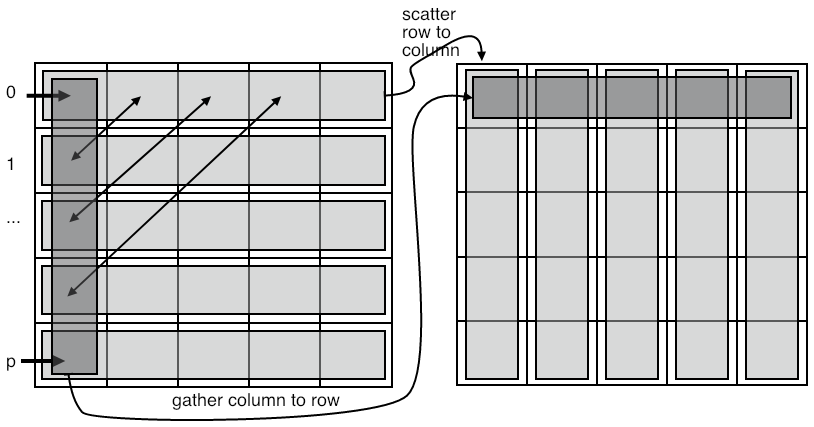
\includegraphics[scale=.4]{alltoall}
  \caption{All-to-all transposes data}
  \label{fig:alltoall}
\end{figure}

The all-to-all operation can be considered as a data transpose. For
instance, assume that each process knows how much data to send to
every other process. If you draw a connectivity matrix of size $P\times P$,
denoting who-sends-to-who, then the send information can be put in
rows:
\[ \forall_i\colon C[i,j]>0\quad\hbox{if process $i$ sends to process $j$}. \]
Conversely, the columns then denote the receive information:
\[ \forall_j\colon C[i,j]>0\quad\hbox{if process $j$ receives from process $i$}. \]

The typical application for such data transposition is in the \ac{FFT}
algorithm, where it can take tens of percents of the running time on
large clusters.

We will consider
another application of data transposition, namely \indexterm{radix sort},
but we will do that in a couple of steps. First of all:

\begin{exercise}
  \label{ex:radixsort1}
  In the initial stage of \indextermsub{radix}{sorting}, each process
  considers how many elements to send to every other process.
  Use \indexmpishow{MPI_Alltoall} to derive from this how many
  elements they will receive from every other process.
\end{exercise}

\index{transpose!and all-to-all|)}

\Level 1 {All-to-all-v}

The major part of the \indexterm{radix sort} algorithm consist
of every process sending some of its elements to
each of the other processes.

\begin{exercise}
  \label{ex:radixsort2}
  The actual data shuffle of a \indextermsub{radix}{sort} can be done
  with \indexmpishow{MPI_Alltoallv}. Finish the code of
  exercise~\ref{ex:radixsort1}.
\end{exercise}

\Level 0 {Reduce-scatter}
\label{sec:reducescatter}

There are several MPI collectives that are functionally equivalent to
a combination of others. You have already seen \indexmpishow{MPI_Allreduce} which
is equivalent to a reduction followed by a broadcast. Often such
combinations can be more efficient than using the individual calls;
see~\HPSCref{sec:collective}.

Here is another example: \indexmpishow{MPI_Reduce_scatter} is equivalent
to a reduction on an array of data (meaning a pointwise reduction on each
array location) followed by a scatter of this array to the individual 
processes.

\begin{figure}[ht]
  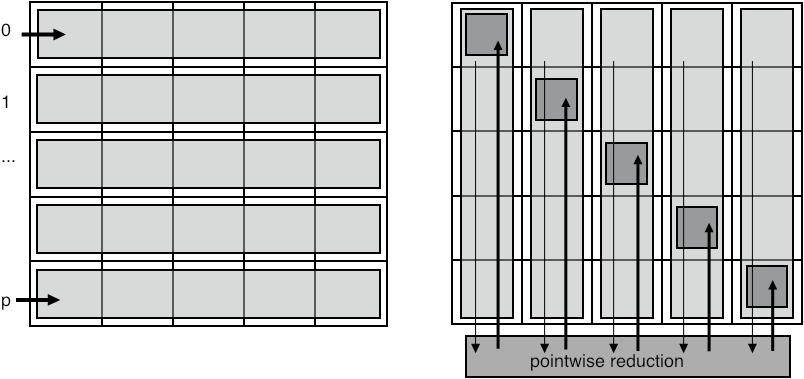
\includegraphics[scale=.4]{reducescatter}
  \caption{Reduce scatter}
  \label{fig:reducescatter}
\end{figure}

We will discuss this routine,
or rather its variant \indexmpixref{MPI_Reduce_scatter_block}{MPI_Reduce_scatter},
using an important example: the
\indextermsub{sparse}{matrix-vector product}
(see~\HPSCref{sec:spmvp-performance} for background information).
Each process contains one or more matrix rows, so by looking at indices
the process can decide what other processes it needs
to receive data from,
that is, each process knows how many messages it will receive,
and from which processes.
The problem is for a process to find out what other processes 
it needs to send data to.

Let's set up the data:
%
\cverbatimsnippet[examples/mpi/c/reducescatter.c]{reducescatterdata}

Each process creates an array of ones and zeros, describing who
it needs data from.
Ideally, we only need the array \lstinline+procs_to_recv_from+
but initially we need the (possibly much larger) array
\lstinline+i_recv_from_proc+.

Next, the \indexmpishow{MPI_Reduce_scatter_block} call then
computes, on each process, how many messages it needs to send.
%
\cverbatimsnippet[examples/mpi/c/reducescatter.c]{reducescattercall}

We do not yet have the information to which processes to send.
For that, each process sends a zero-size message to
each of its senders.
Conversely, it then does a receive to with \lstinline+MPI_ANY_SOURCE+
to discover who is requesting data from it.
The crucial point to the \lstinline+MPI_Reduce_scatter_block+ call
is that, without it, a~process would not know how many
of these zero-size messages to expect.

\cverbatimsnippet[examples/mpi/c/reducescatter.c]{reducescattertest}

The \indexmpiref{MPI_Reduce_scatter} call is more general:
instead of indicating the mere presence of a message
between two processes,
by having individual receive counts one can, for instance,
indicate the size of the messages.

We can look at reduce-scatter as a limited form of the all-to-all data
transposition discussed above (section~\ref{sec:alltoall-transpose}).
Suppose that the matrix~$C$ contains only~$0/1$, indicating
whether or not a messages is send, rather than the actual amounts.
If a receiving process only needs to know how many messages to
receive, rather than where they come from, it is enough to know the
column sum, rather than the full column (see figure~\ref{fig:reducescatter}).

Another application of the reduce-scatter mechanism is in the
dense matrix-vector product, if a two-dimensional data distribution
is used.

\Level 1 {Examples}

An important application of this is establishing an irregular
communication pattern.  Assume that each process knows which
other processes it wants to communicate with; the problem is to
let the other processes know about this.
The solution is to use \indexmpishow{MPI_Reduce_scatter} to find out how many processes
want to communicate with you
\cverbatimsnippet[examples/mpi/c/reducescatter.c]{reducescattercall}
and then wait for precisely that many messages
with a source value of \indexmpishow{MPI_ANY_SOURCE}.
\cverbatimsnippet[examples/mpi/c/reducescatter.c]{reducescattertest}

Use of \indexmpishow{MPI_Reduce_scatter} to implement the two-dimensional
matrix-vector product.
Set up separate row and column communicators with
\indexmpishow{MPI_Comm_split}, use \indexmpishow{MPI_Reduce_scatter} to combine
local products.
%
\cverbatimsnippet[examples/mpi/c/mvp2d.c]{mvp2d}

\Level 0 {Barrier}
\label{sec:barrier}

A~barrier call,
%
\indexmpiref{MPI_Barrier}
%
is a
routine that blocks all processes until they have all reached the barrier
call. Thus it achieves time synchronization of the processes.

This call's simplicity is contrasted with its usefulness, which
is very limited. It is almost never necessary to synchronize processes
through a barrier: for most purposes it does not matter if processors
are out of sync. Conversely, collectives (except the new non-blocking
ones; section~\ref{sec:mpi3collect}) introduce a barrier of sorts themselves.

